\documentclass[a4paper]{article}

\usepackage[english,russian]{babel}
\usepackage{hyperref}
\hypersetup{
    colorlinks,
    citecolor=black,
    filecolor=black,
    linkcolor=black,
    urlcolor=blue
}
\usepackage{float}
\usepackage{subcaption}
\usepackage[utf8]{inputenc}
\usepackage[12pt]{extsizes}
\usepackage{physics}
\usepackage{graphicx}
\graphicspath{{../misc/}}
\usepackage{setspace,amsmath}
\usepackage[left=20mm, top=15mm, right=15mm, bottom=15mm, nohead, footskip=10mm]{geometry}
\usepackage{wrapfig}

\usepackage[backend=biber]{biblatex}
\addbibresource{lit.bib}

\begin{document} 

\begin{center}
    \hfill \break
    ФЕДЕРАЛЬНОЕ ГОСУДАРСТВЕННОЕ БЮДЖЕТНОЕ ОБРАЗОВАТЕЛЬНОЕ 

    УЧРЕЖДЕНИЕ ВЫСШЕГО ОБРАЗОВАНИЯ

    «МОСКОВСКИЙ ГОСУДАРСТВЕННЫЙ УНИВЕРСИТЕТ

    имени М.В.ЛОМОНОСОВА» 

    \hfill \break
    \normalsize{ФИЗИЧЕСКИЙ ФАКУЛЬТЕТ}\\
    \hfill \break
    \normalsize{КАФЕДРА ОБЩЕЙ ФИЗИКИ И МОЛЕКУЛЯРНОЙ ЭЛЕКТРОНИКИ}\\
    \hfill\break
    \hfill \break
    \hfill \break
    \large\textbf{«МОДЕЛИРОВАНИЕ РАСПОЗНАВАНИЯ ОБРАЗОВ НА ОСНОВЕ ИМПУЛЬСНЫХ НЕЙРОННЫХ СЕТЕЙ С КОНКУРЕНЦИЕЙ ЛОКАЛЬНЫХ РЕЦЕПТИВНЫХ ПОЛЕЙ»}\\
    \hfill \break

\end{center}

\begin{flushright}

    Выполнил студент:

    406 группа

    Гафни Д.
    
    $\underset{\text{подпись студента}}{\underline{\hspace{0.3\textwidth}}}$

    \hfill\break

    Научный руководитель:

    Королёва А.В.

    $\underset{\text{подпись научного руководителя}}{\underline{\hspace{0.3\textwidth}}}$
    
    \hfill\break
    
    Научный консультант:

    Дёмин В.А.

    $\underset{\text{подпись научного консультанта}}{\underline{\hspace{0.3\textwidth}}}$

\end{flushright}

\begin{center}

\vfill
Москва\\
2020
\end{center}

\thispagestyle{empty} 

\pagebreak

\tableofcontents

\section{Описание проблемы}
Импульсные (спайковые) нейронные сети (СНС) являются перспективным нейроморфным алгоритмом, биологически корректно моделируя взаимодействия нейронов мозга. Наибольший интерес СНС представляют для решения задач в реальном времени (принятие решений, распознавание образов), так как могут быть реализованы на специализированном вычислительно- и энергоэффективном мемристорном нейрочипе, так как 

Стандартные методы обучения весов связей, применяющиеся в формальных нейронных сетях (метод обратного распространения ошибки) не представляется возможным применять к СНС из-за их дискретной и распределенной во времени природы. Таким образом, исследование алгоритмов обучения СНС представляется важной задачей.

Современные формальные нейронные сети отлично справляются со многими задачами машинного обучения \cite{pmlr-v28-wan13}. Однако их обучение - трудоемкий процесс, требующий больших вычислительных ресурсов. Обычно обучение ведется на десятках и сотнях тысячах примеров и может занимать месяцы. Как само обучение, так и последующее применение формальных нейросетевых алгоритмов далеки от эффективности. Это связано как с физически раздельным хранением значений весов и активаций нейронов, так и с самими вычислениями, которые носят тензорный характер. Современные процессоры не оптимизированы для подобных вычислений. Гораздо лучше процессоров для этих задач подходят GPU - архитектуры, изначально созданные для работы с компьютерной графикой и больше оптимизированные для тензорных вычислений, однако и они не дают желаемого результата. Число параметров в современных формальных нейронных сетях может достигать сотен миллионов \cite{ManyParams}.

\section{Постановка задачи}
В данной работе:

\begin{enumerate}
 \item Изучается влияние обучения связей конкуренции \cite{MaxActiv1} \cite{MaxActiv2} между нейронами на точность распознавания образов в задаче классификации рукописных изображений цифр (MNIST) при обучении без учителя для архитектуры локально соединенной сети (Locally Connected Spiking Neural Network, LCSNN) \cite{saunders2019locally}
 
 \item Проводится сравнение этой архитектуры со сверточной сетью (Convolution Spiking Neural Network, CSNN) и полносвязной сетью (Fully Connected Spiking Neural Network, FCSNN).

\end{enumerate}

\section{Спайковые нейронные сети}
Спайковая нейронная сеть - модель нейронной сети, элементами которой являются  отдельные нейроны и связи между ними. Каждый нейрон имеет свой виртуальный потенциал, а каждая связь имеет некоторый вес. Нейроны обмениваются дискретными электрическими сигналами (спайками), имеющими очень короткую ($ \approx ~1$ мс) длительность. Входящий спайк носит название пре-спайка, а исходящий - пост-спайка.  Влияние пре-спайков на потенциал нейрона определяется значением веса межнейронной связи. При накоплении потенциала, превышающего определенный порог активации, нейрон сам испускает пост-спайк, а после сбрасывает свое напряжение до некоторого уровня релаксации. При запуске сети активность некоторых входных нейронов задается определенным образом, после чего проводится симуляция на протяжении некоторого времени ($\approx ~250$ мс), много большего длительности спайка.

\section{Моделирование обучения спайковой нейронной сети с конкуренцией локальных рецептивных полей}

\subsection{Описание задачи классификации} 
Для работы была выбрана классическая задача машинного обучения - задача классификации изображений рукописных цифр из набора данных MNIST. MNIST состоит из размеченных обучающей и тестовых выборок объемами 60000 и 10000 изображений. Изображения имеют размер 24x24 пикселя и являются черно-белыми. Из-за необходимости калибровки сетей (\ref{calibration}) обучающая выборка была разбита на 50000 изображений для обучения (обучающая выборка) и 10000 изображений для калибровки (калибровочная выборка).


\begin{wrapfigure}[10]{r}{.5\textwidth} \label{MNIST} 
% \begin{center}
 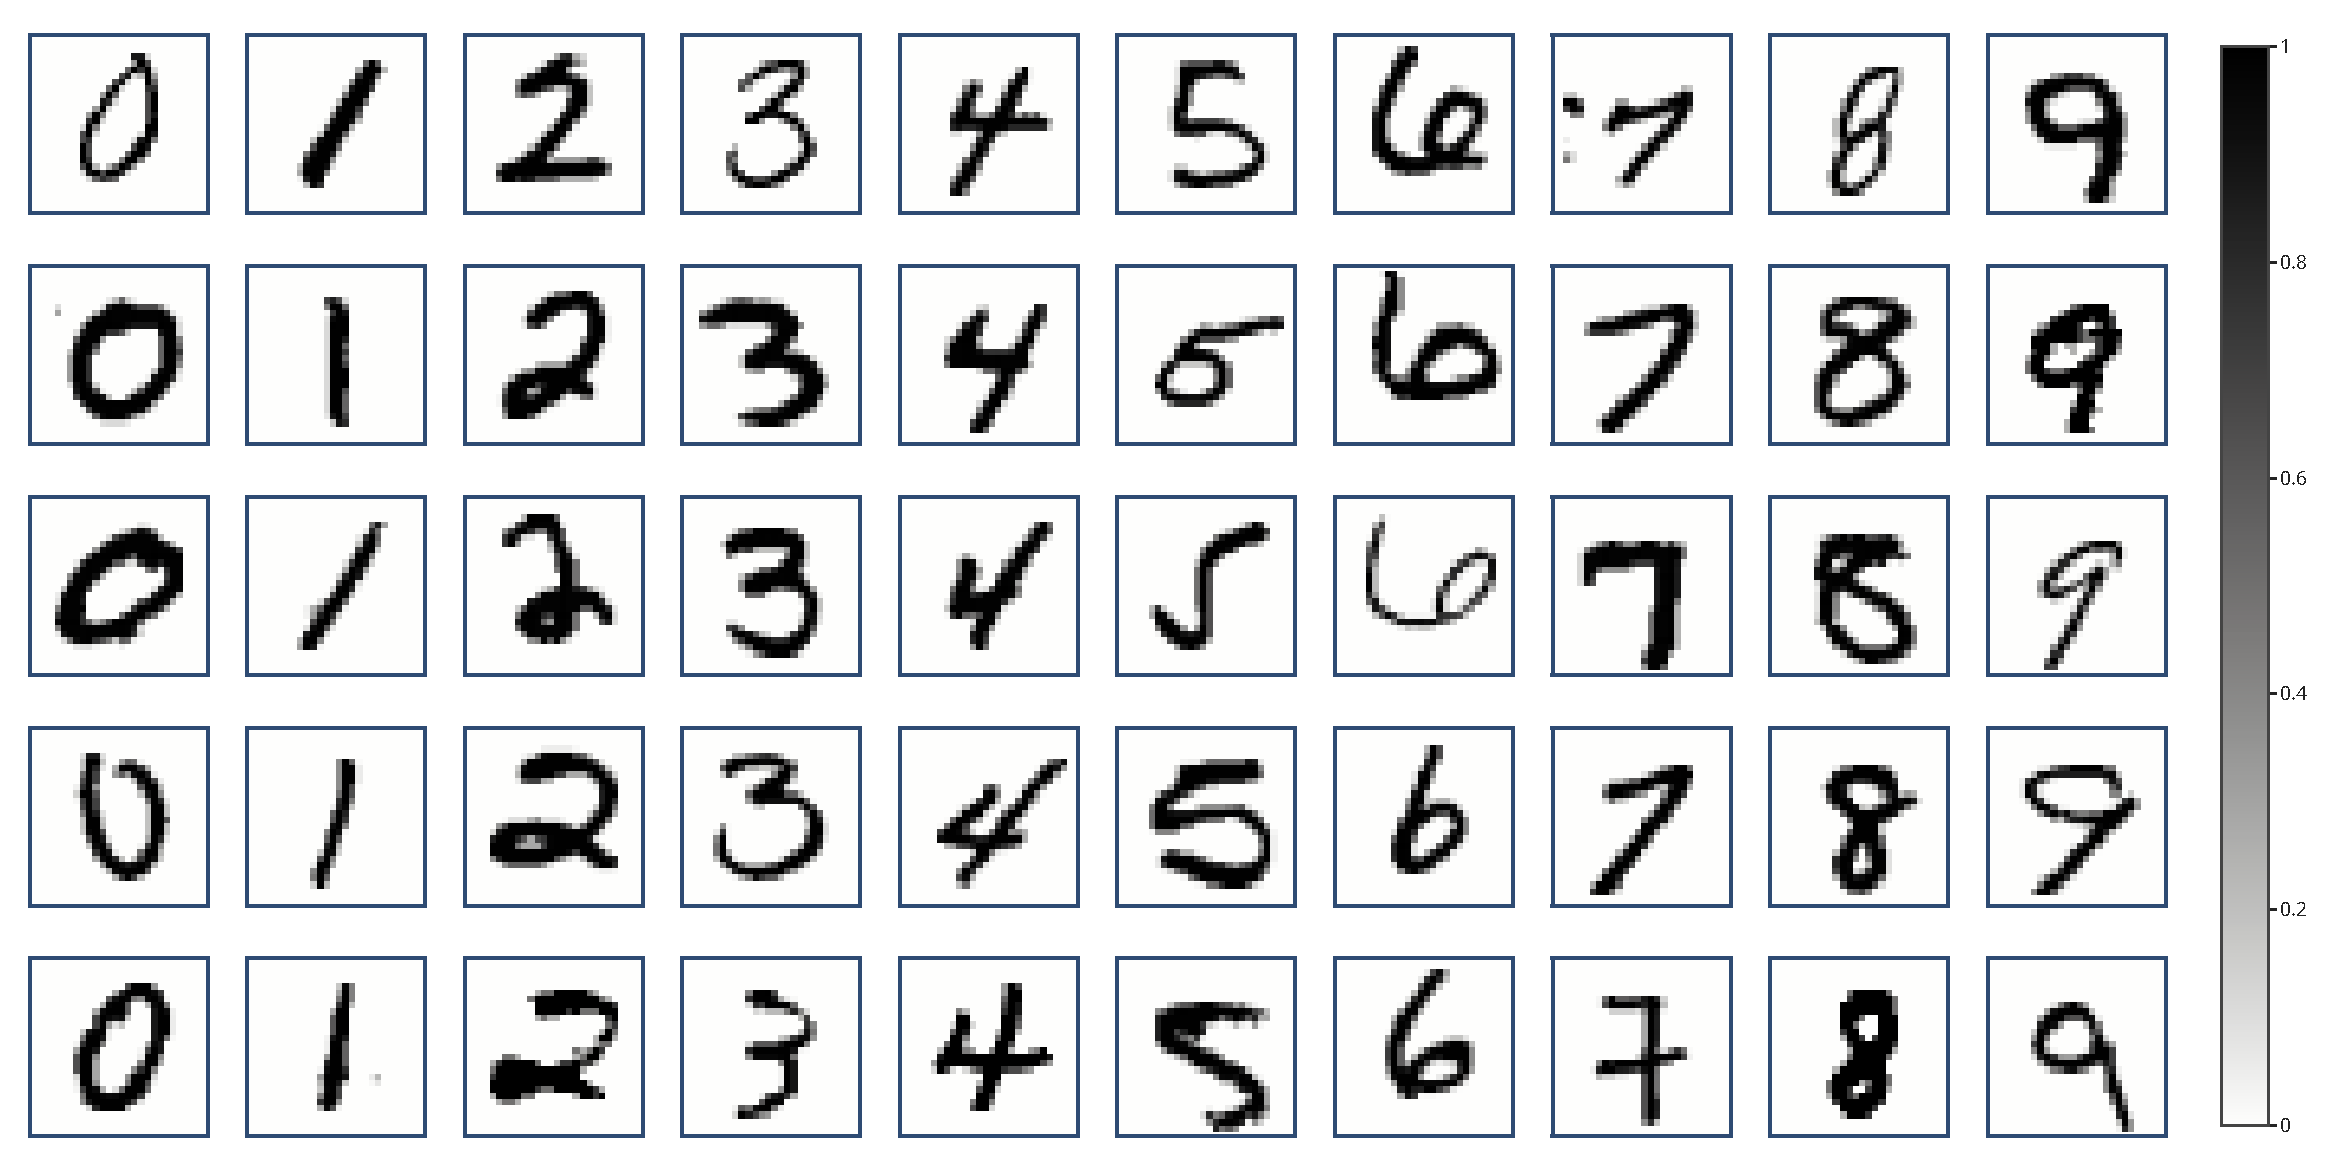
\includegraphics[width=.5\textwidth,keepaspectratio=true]{MNIST.pdf} 
 
 \caption{Изображения MNIST}
% \end{center}
\end{wrapfigure}


В этой работе изображения обрезаются так, что используется только центральная область 20x20 пикселей.\\

\subsection{Особенности архитектуры}
Нейросетевая архитектура LCSNN \cite{saunders2019locally} вдохновлена строением зрительной коры мозга. В отличие от сверточной сети, ее нейроны не имеют общих весов, которые потому и называются локальными.

\begin{wrapfigure}[14]{r}{.5\textwidth} \label{MNIST} 
 \centering
 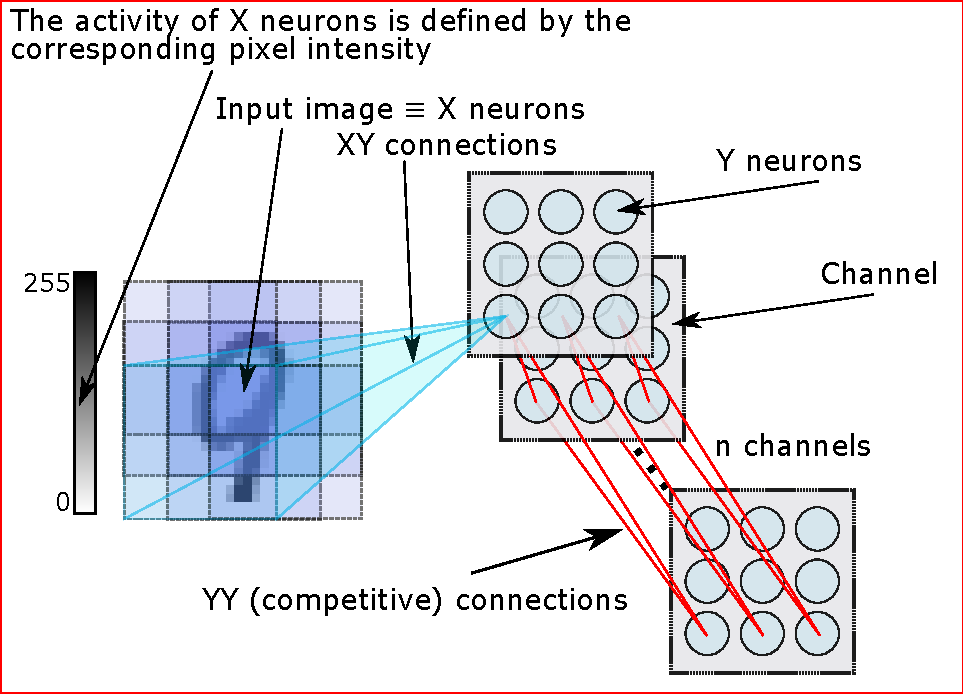
\includegraphics[width=0.5\textwidth]{LCSNN.pdf}
\end{wrapfigure}

Нейроны, имеющие общие рецептивные поля, соединяются связями конкуренции. Такие связи имеют отрицательные веса, а значит, негативно влияют на активность нейрона. Заметим, что нейроны, не имеющие общего рецептивного поля (а значит, реагирующие на разные области изображения) не конкурируют между собой.\\

Для обучения всех сетей в этой работе используется правило STDP \cite{STDP}. Согласно этому правилу обучения, также заимствованному из нейронов мозга, связь между нейронами усиляется, если пост-спайк этой связи часто случается после пре-спайка, и ослабевает, если происходит обратное.

\subsection{Обучение связей $XY$}
При обучении связей $XY$ 

\begin{wrapfigure}[13]{r}{.45\textwidth}
\centering
\begin{subfigure}{0.2\textwidth}
    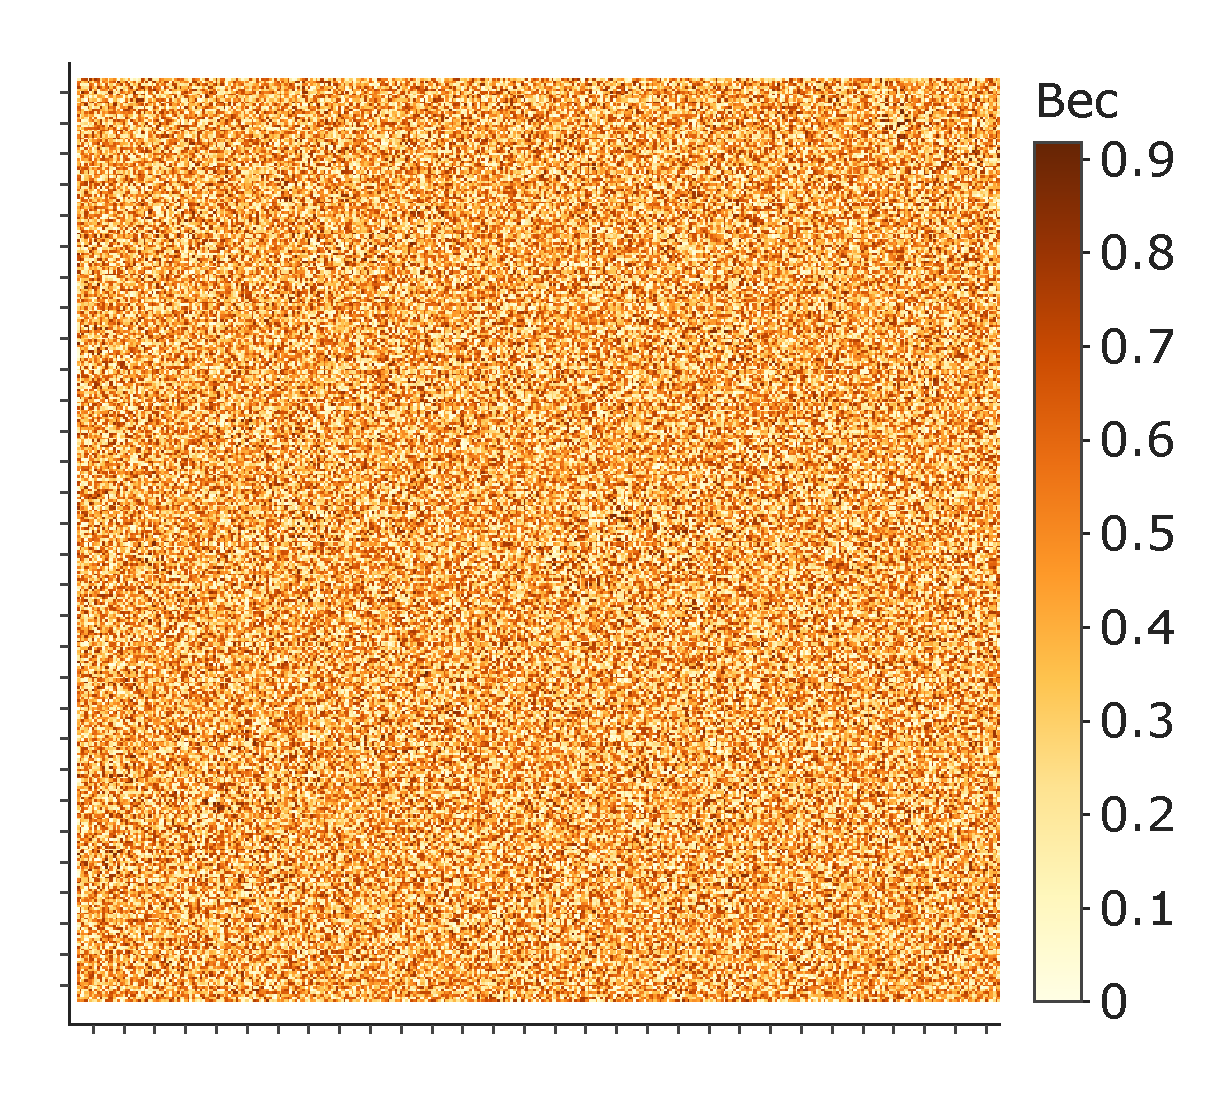
\includegraphics[width=\textwidth,keepaspectratio=true]{weights_XY_untrained_ru.pdf}
    \caption{Веса перед обучением}
\end{subfigure}
\begin{subfigure}{0.2\textwidth}  \label{weights_XY}
    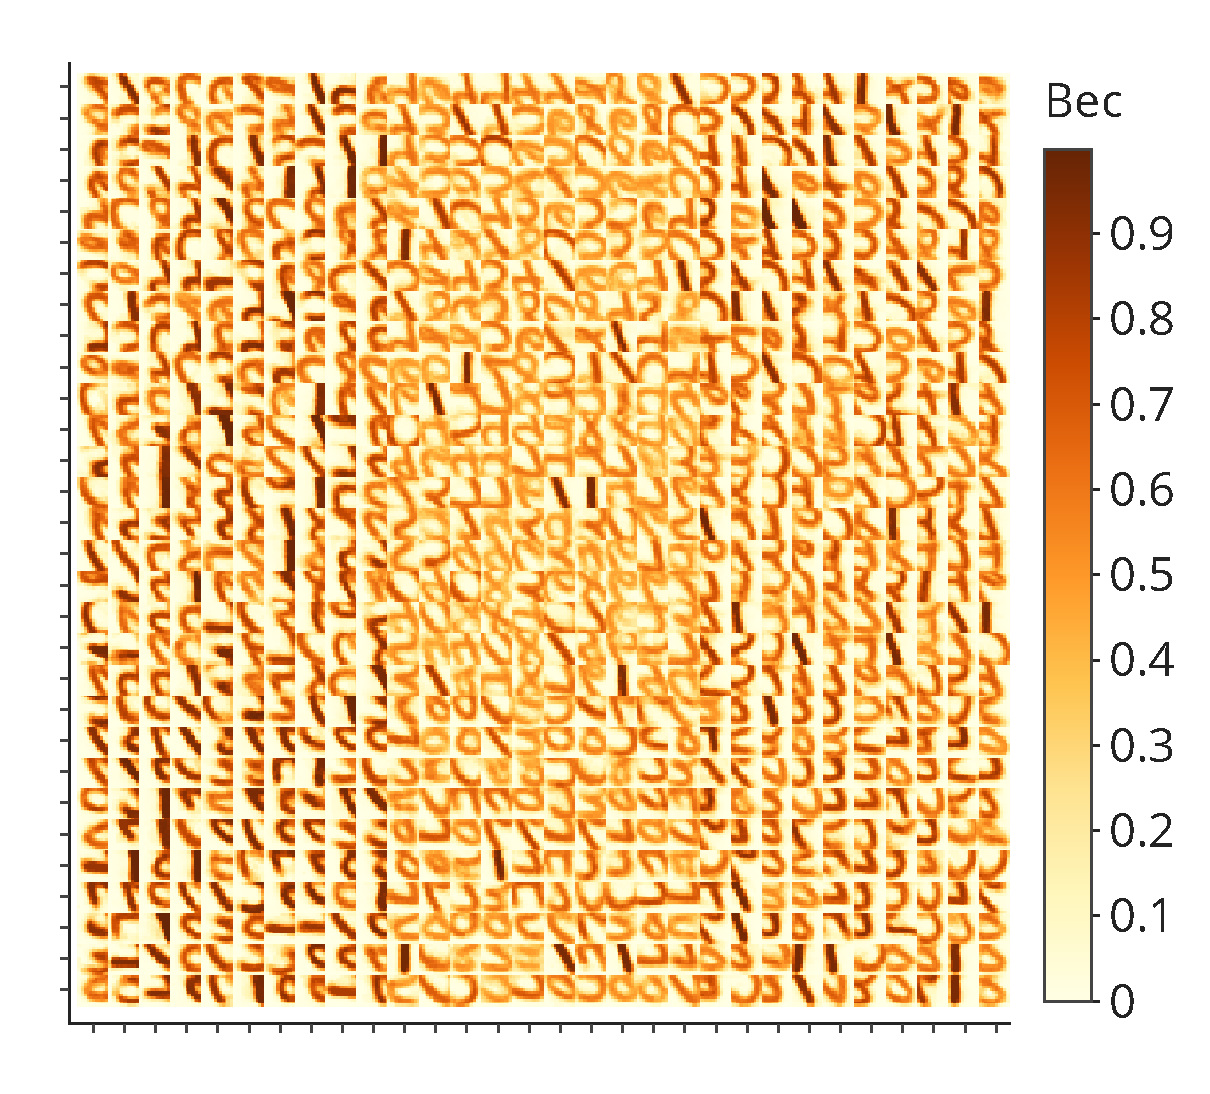
\includegraphics[width=\textwidth,keepaspectratio=true]{weights_XY_ru.pdf}
    \caption{Веса после обучения}
\end{subfigure}
\caption{Визуализация весов $XY$ связей. Каждый квадратик соответствует весам одного $Y$ нейрона.}
\end{wrapfigure}

\subsubsection{Интерпретация активности спайковой нейронной сети}
Для интерпретации активности нейронов $Y$ слоя сети использовалось несколько методов.


\paragraph{Калибровка голосов} \label{calibration}
Для первых трех методов необходимо произвести калибровку голосов нейронов. Каждому нейрону $Y$ слоя ставится в соответствие 10 чисел (голосов) для каждого возможного класса цифр (от 0 до 9). Голос вычисляется как среднее число спайков данного нейрона в ответ на демонстрацию сети данной цифры. Для всех сетей использовалась калибровка на 10000 примерах из калибровочной выборки. Заметим, что калибровка не является частью обучения сети, так как она входит лишь в алгоритм интерпретации поведения сети. Эти голоса используются как мера уверенности нейрона в каждом из классов. После демонстрации изображения сети подсчитывается общее количество спайков для каждого нейрона $Y$ слоя.

\begin{wrapfigure}[17]{H}{.5\textwidth}
\centering
\begin{subfigure}{.5\textwidth}
    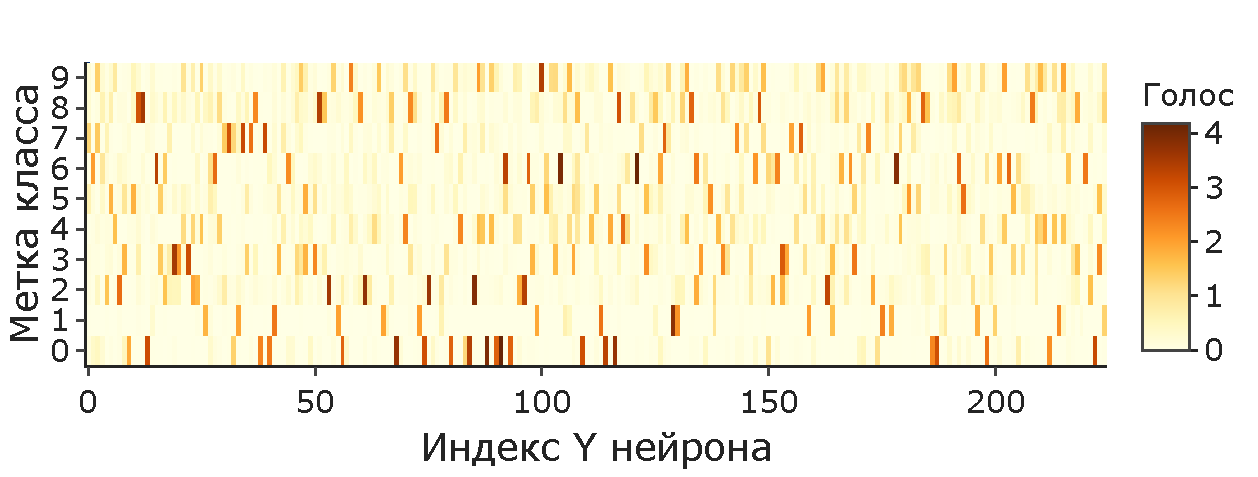
\includegraphics[width=\textwidth,keepaspectratio=true]{votes_ru.pdf}
    \caption{Голоса нейронов $Y$ слоя.}
\end{subfigure} 
\begin{subfigure}{.5\textwidth} 
    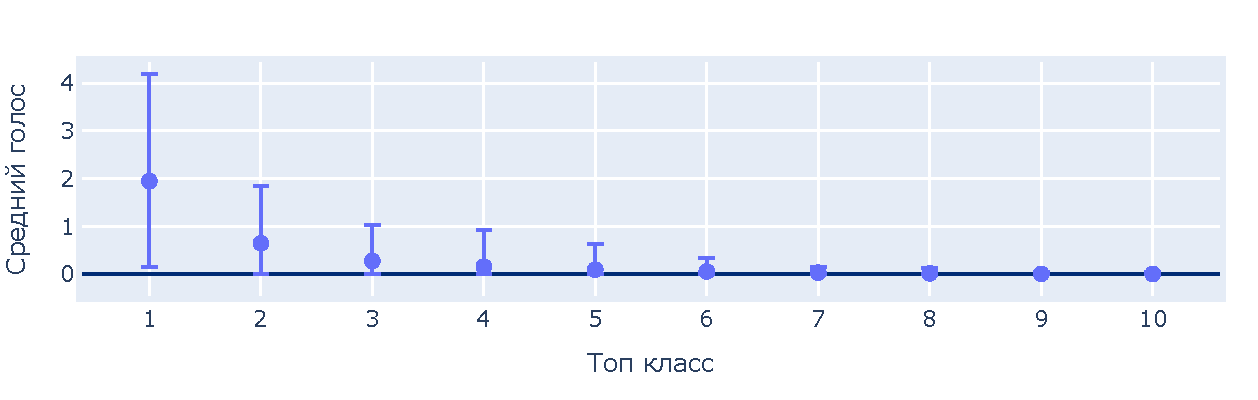
\includegraphics[width=\textwidth,keepaspectratio=true]{votes_distribution_ru.pdf}
    \caption{Среднее значение голоса для топ-n класса, где топ-1 - класс с максимальным голосом нейрона, топ-10 - класс с минимальным голосом нейрона.}
\end{subfigure}
\caption{Визуализация голосов нейронов $Y$ слоя. Высокие значения соответствуют большой специализации нейрона на соответствующем классе.}
\end{wrapfigure}

Далее \textit{результатом} будем называть произведение количества спайков нейрона на голос.

\paragraph{Общее голосование}
Ответом сети считается класс с максимальным  \textit{результатом} среди всех нейронов.

\paragraph{Голосование патчей}
Для каждого рецептивного поля ищется нейрон с максимальным \textit{результатом}. Ответом сети считается класс с максимальным результатом среди этих нейронов.

\paragraph{Отбор по спайкам}
Для каждого рецептивного поля ищется нейрон с максимальным количеством спайков. Ответом сети считается класс с максимальным результатом среди этих нейронов.

\paragraph{Линейный классификатор}
Суммы спайков нейронов $Y$ слоя используются для обучения линейного классификатора. Для обучения классификатора также используется калибровочная выборка.

\paragraph{Оценка алгоритма интерпретации}
Для оценки работы алгоритма интерпретации используется точность - отношение количества верно распознанных цифр к размеру тестовой выборки. В этой работе во всех случаях размер тестовой выборки составляет 10000. 

\begin{wrapfigure}[15]{r}{.45\textwidth}
\centering
 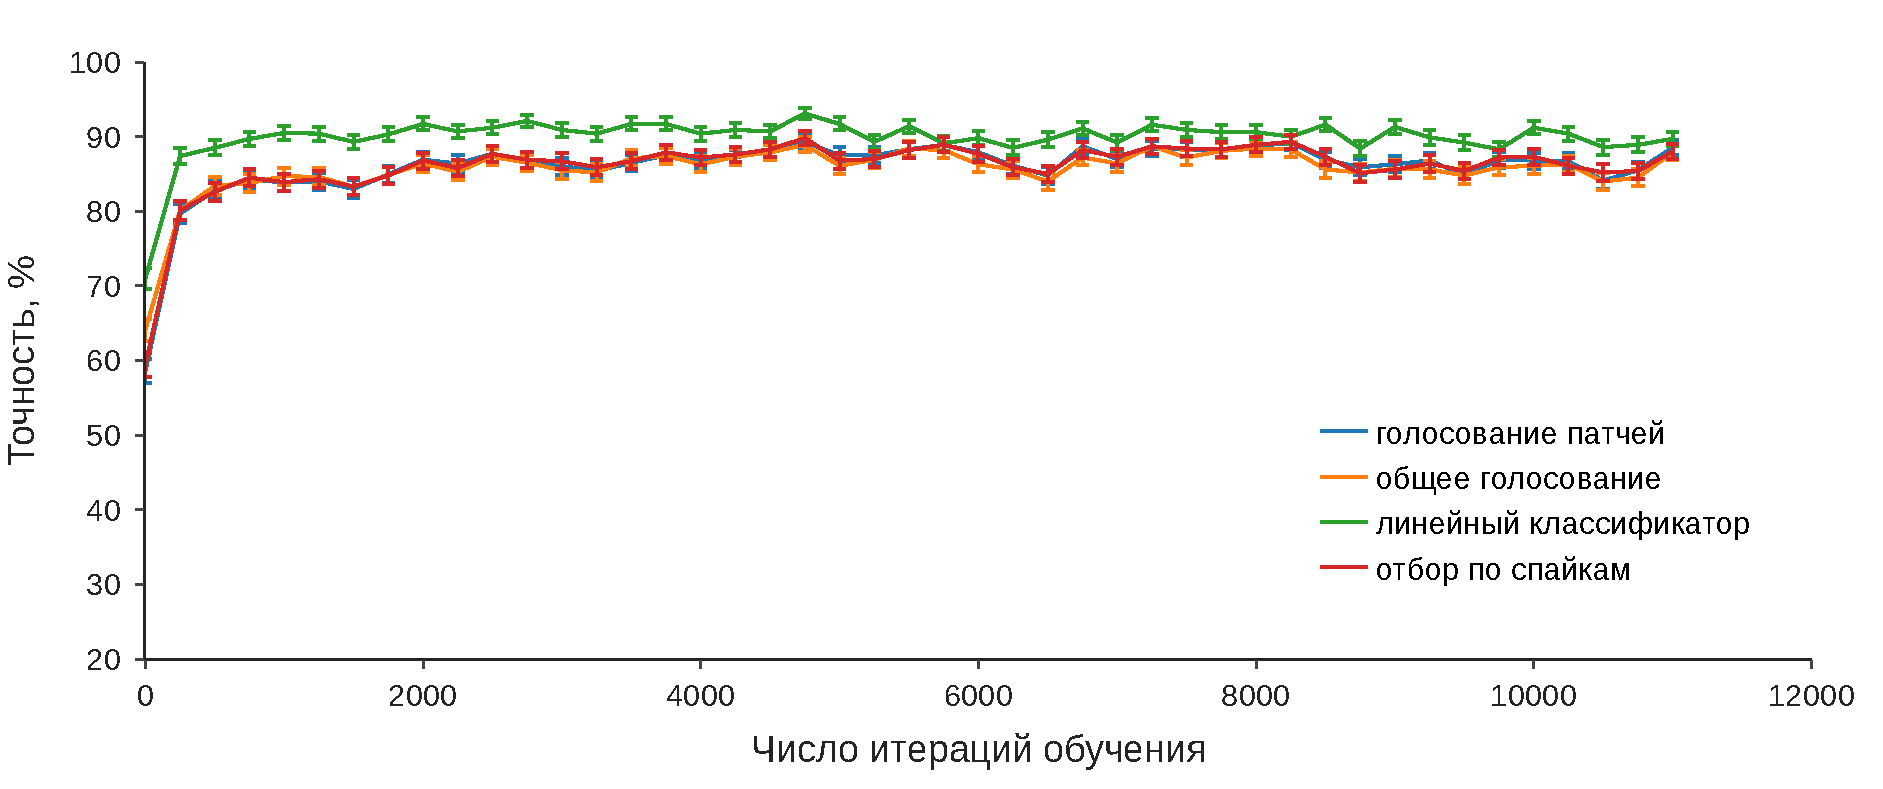
\includegraphics[width=.45\textwidth,keepaspectratio=true]{LCSNN_learning_rate_ru.pdf}
 \caption{LCSNN отличаются большой скоростью обучения. Через несколько тысяч итераций точность распознавания выходит на плато насыщения, после чего уже не возрастает. Видно, что три метода голосования в целом не отличаются по точности, а линейный классификатор значительно превосходит их все.}
\end{wrapfigure}


\subsection{Сравнение эффективности операции свертки и локального рецептивного поля}
Были проведены эксперименты по измерению точности сеткй с различными архитектурами. Из-за очень высоких вычислительных нагрузок не ставилось задачи по нахождению параметров, идеально обеспечивающих максимальную точность для каждой архитектуры. Эти параметры были подобраны приблизительно, поэтому могли не попасть в максимум точности, однако величина расхождения не превышает 1-2\%. Было протестировано несколько конфигураций для локально соединенных и для сверточных сетей, а также произведено сравнение со стандартной полносвязной сетью (также имеющей связи конкуренции). Видно, что локально соединенная сеть превосходит сверточную по точности при одинаковом числе нейронов (сравнивается количество нейронов $Y$ слоя). 

\begin{table}[H]
 \caption{Результаты сравнения различных архитектур спайковых нейронных сетей. Для каждой сети точность измерялась $N=5$ раз. В таблице указаны средние значения и стандартное отклонение для точности.}
\begin{center}
\begin{tabular}{|l|l|l|l|l|l|l|}
\hline
Архитектура & Фильтры & Ядро & Веса & Нейроны & Точность & Погрешность\\
\hline
{LCSNN} & {100} & {12} & {449100} & {900} & {0.8752} & {0.0090}\\
\hline
{LCSNN} & {100} & {8} & {798400} & {1600} & {0.8285} & {0.0021}\\
\hline
{LCSNN} & {25} & {12} & {95400} & {225} & {0.8005} & {0.0102}\\
\hline
{LCSNN} & {25} & {8} & {169600} & {400} & {0.7360} & {0.0103}\\
\hline
{CSNN} & {100} & {8} & {11350} & {1600} & {0.7736} & {0.0188}\\
\hline
{CSNN} & {25} & {12} & {3900} & {225} & {0.6577} & {0.0067}\\
\hline
{CSNN} & {25} & {8} & {1900} & {400} & {0.5807} & {0.0117}\\
\hline
{FCSNN} & {100} & {20} & {44950} & {100} & {0.7340} & {0.0866}\\
\hline
\end{tabular}
\end{center}
\end{table}



\subsection{Обучение связей $YY$ (конкуренции)}
Связи $YY$ очень сильно влияют на обучение связей $XY$. Большие по модулю значения способствуют вариативности в обучении $Y$ нейронов, так для каждого рецептивного поля одновременно активными не могут быть нейроны, имеющие схожие веса $XY$, а малые по модулю значения не позволяют нейронам специализироваться.

\begin{wrapfigure}[13]{r}{.45\textwidth}
\centering
\begin{subfigure}{0.2\textwidth}
    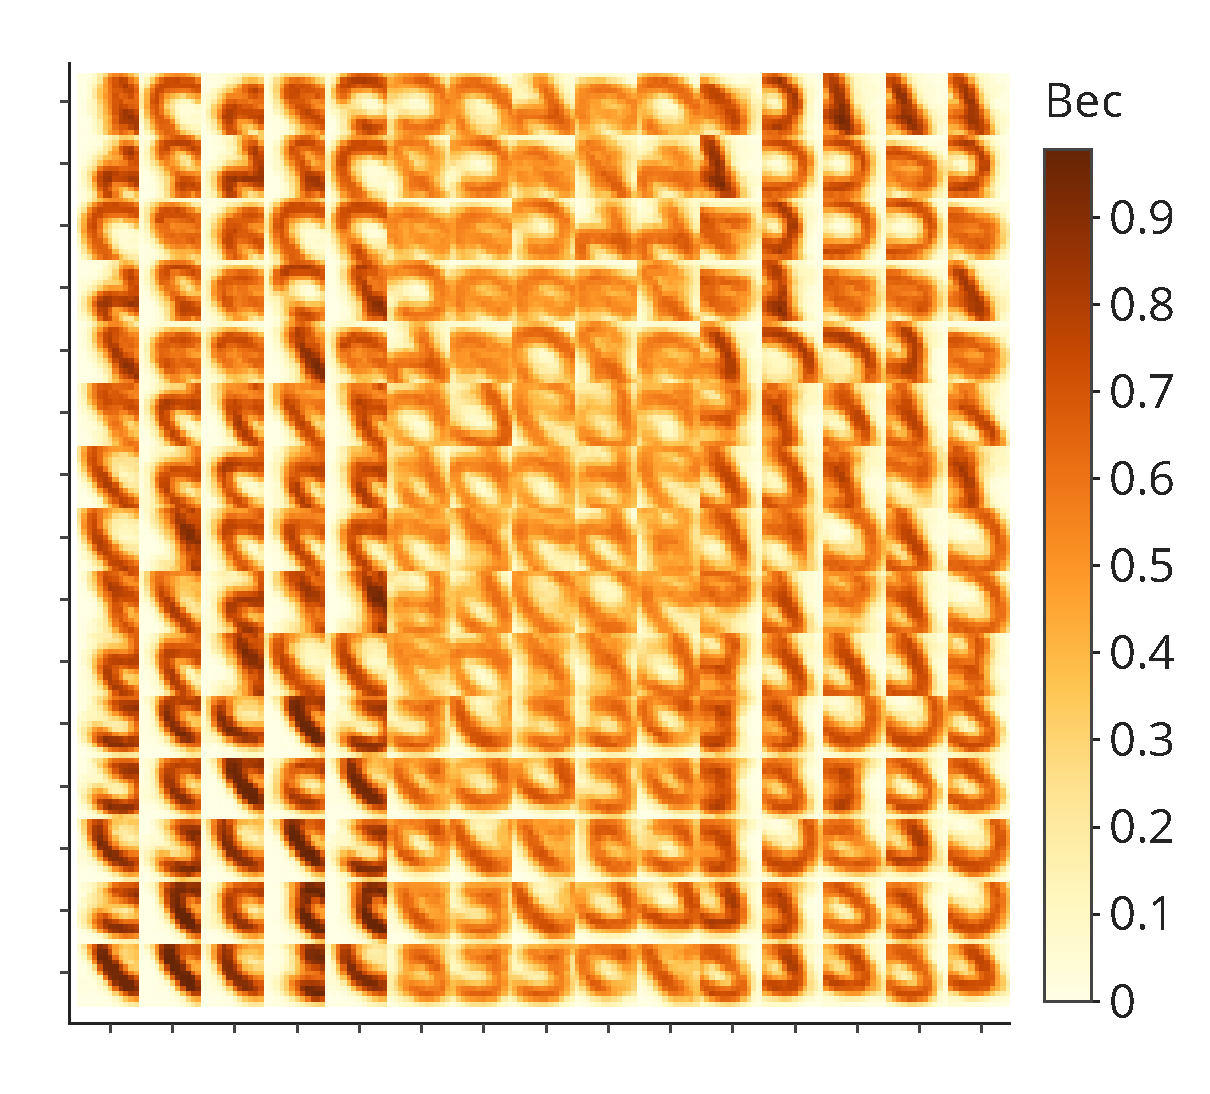
\includegraphics[width=\textwidth,keepaspectratio=true]{weights_XY_bad_ru.pdf}
    \caption{Слабо специализированные веса,\\ вес конкуренции равен $-10$}
\end{subfigure}
\begin{subfigure}{0.2\textwidth}
    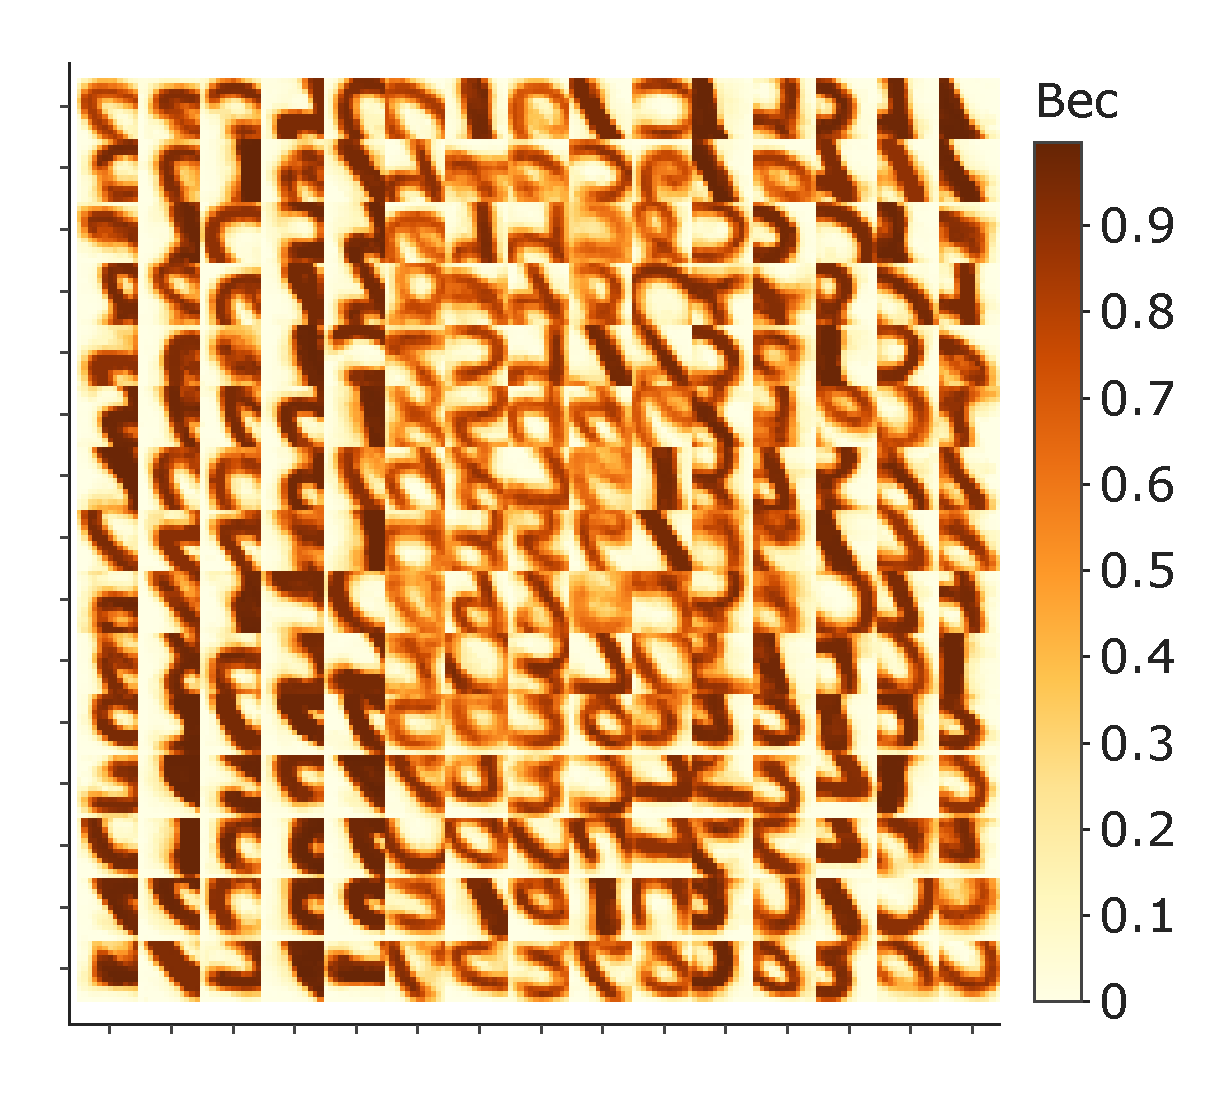
\includegraphics[width=\textwidth,keepaspectratio=true]{weights_XY_good_ru.pdf}
    \caption{Специализированные веса,\\ вес конкуренции равен $-100$}
\end{subfigure}
\caption{Влияние конкуренции на обучение $XY$ связей}
\end{wrapfigure}

Все сети до этого момента имели фиксированные веса конкуренции. Было обнаружено, что обучение весов конкуренции позволяет повысить точность сети. При помощи варьирования параметров STDP были получены различные распределения весов конкуренции.

\begin{wrapfigure}[12]{r}{.45\textwidth}
\centering
\begin{subfigure}{0.2\textwidth}
    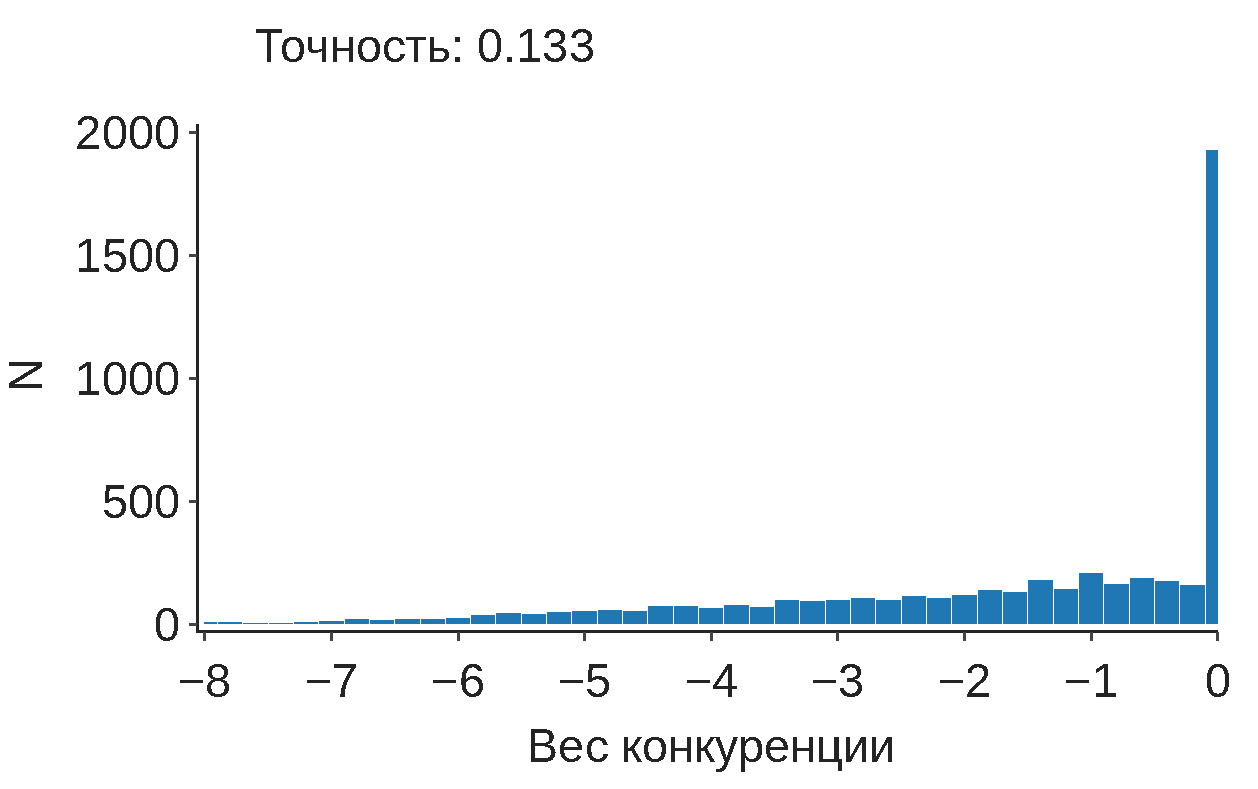
\includegraphics[width=\textwidth,keepaspectratio=true]{competition_distribution_worst_ru.pdf}
    \caption{Очень слабая конкуренция}
\end{subfigure}
\begin{subfigure}{0.2\textwidth}
    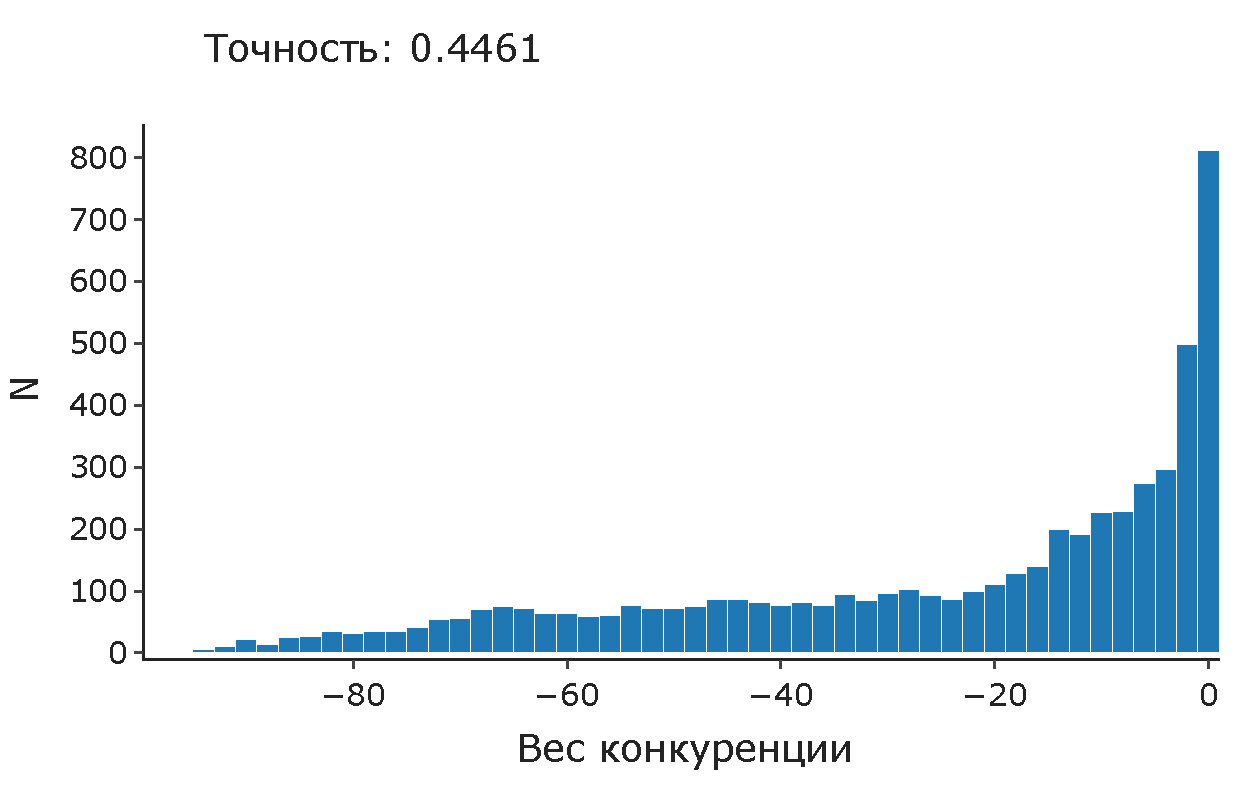
\includegraphics[width=\textwidth,keepaspectratio=true]{competition_distribution_medium_bad_ru.pdf}
    \caption{Слабая конкуренция}
\end{subfigure}
\\
\begin{subfigure}{0.2\textwidth}
    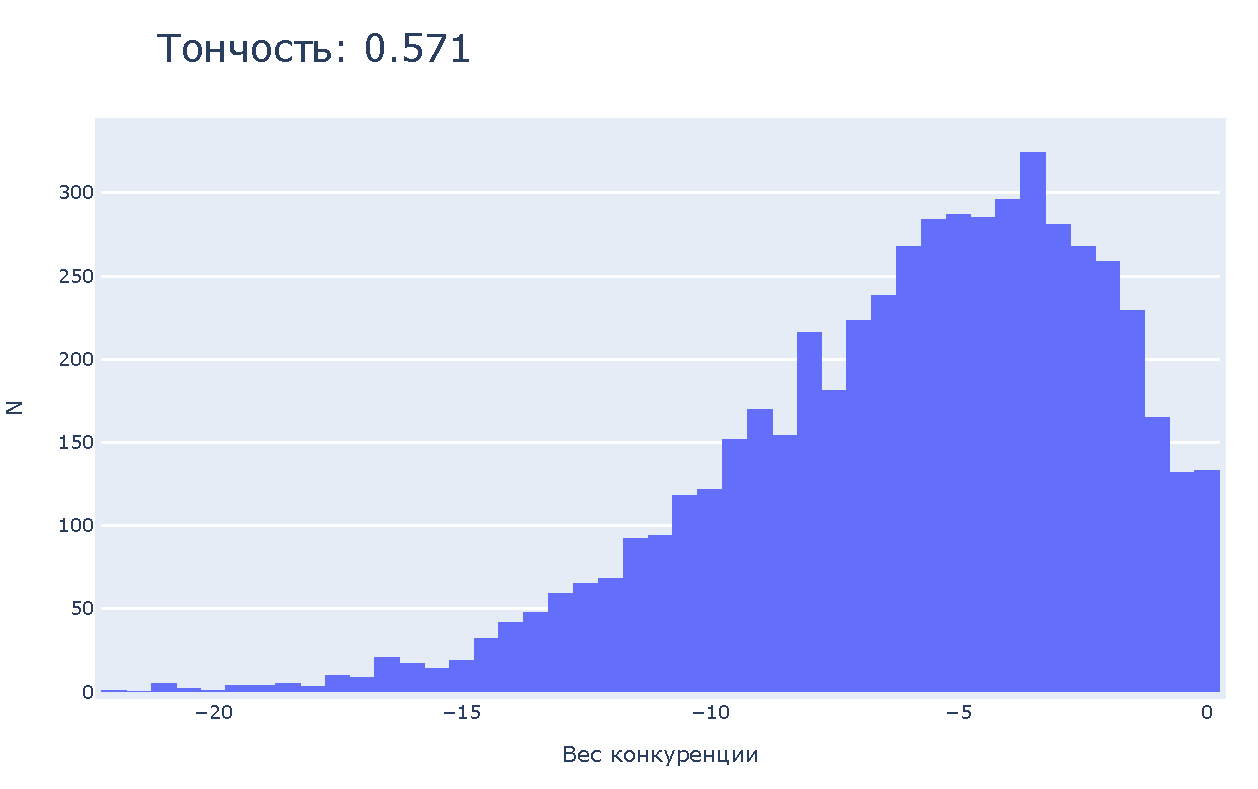
\includegraphics[width=\textwidth,keepaspectratio=true]{competition_distribution_medium_good_ru.pdf}
    \caption{Средняя конкуренция} 
\end{subfigure}
\begin{subfigure}{0.2\textwidth}
    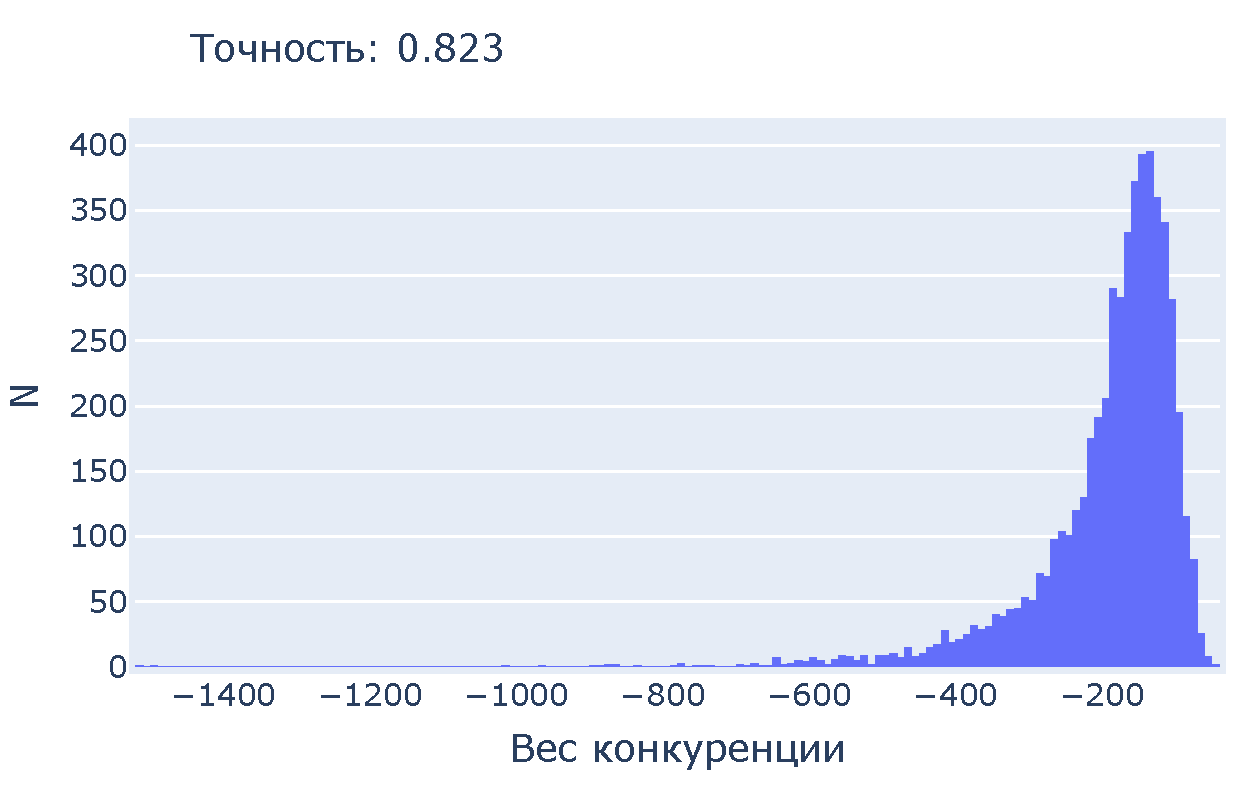
\includegraphics[width=\textwidth,keepaspectratio=true]{competition_distribution_best_ru.pdf}
    \caption{Сильная конкуренция}
\end{subfigure}
\caption{Различные распределения весов конкуренции}
\end{wrapfigure}

Видно, что точность сети повышается при тяготении распределения весов конкуренции в сторону больших по модулю значений. Заметим, что целью являлось не нахождение параметров сети, обеспечивающих максимальную точность, а исследования влияния обучения или не-обучения конкуренции на точность сети с данной конфигурацией остальных параметров.

Примечательно, что не все связи $YY$ получают большие по модулю значения. Это объясняется тем, что нейроны, специализирующиеся на значительно разных элементах, не нуждаются в конкуренции, так как они не проявляют высокую активность одновременно.

\section{Выводы}
Было обнаружено, что обучение связей конкуренции нейронов, имеющих общие рецептивные поля, позволяет добиться большей точности распознавания изображений по сравнению с той же архитектурой, но с необучаемыми связями конкуренции. Также было показано, что LCSNN имеет преимущество над CSNN как по скорости обучения, так и по точности распознавания. Таким образом, локально соединенная сеть – перспективная нейросетевая архитектура, превосходящая классические алгоритмы в точности распознавания изображений при обучении без учителя, и подходит для реализации на вычислительном мемристорном нейрочипе.

\printbibliography

\end{document}  
